\pdfminorversion=4 % for acroread
%\documentclass[aspectratio=169,t,xcolor={usenames,dvipsnames}]{beamer}
\documentclass[aspectratio=169,t,handout,xcolor={usenames,dvipsnames}]{beamer}
\usepackage{../beamerstyle}
\usepackage{dsfont}
\usepackage{bm}
\usepackage[english]{babel}
\usepackage[utf8]{inputenc}
\usepackage{graphicx}
\usepackage{algorithm}
\usepackage[ruled,vlined,algo2e,linesnumbered]{algorithm2e}
%\usepackage[boxed,vlined]{algorithm2e}
\usepackage{hyperref}
\usepackage{booktabs}
\usepackage{mathtools}

\usepackage{amsmath,amssymb}
\usepackage{listings}
\lstset{frame=lines,framesep=3pt,numbers=left,numberblanklines=false,basicstyle=\ttfamily\small}

\usepackage{subfig}
\usepackage{multicol}
%\usepackage{appendixnumberbeamer}
%
\usepackage{tcolorbox}

\usepackage{pgfplots}
\usepackage{tikz}
\usetikzlibrary{trees} 
\usetikzlibrary{shapes.geometric}
\usetikzlibrary{positioning,shapes,shadows,arrows,calc,mindmap}
\usetikzlibrary{positioning,fadings,through}
\usetikzlibrary{decorations.pathreplacing}
\usetikzlibrary{intersections}
\usetikzlibrary{positioning,fit,calc,shadows,backgrounds}
\pgfdeclarelayer{background}
\pgfdeclarelayer{foreground}
\pgfsetlayers{background,main,foreground}
\tikzstyle{activity}=[rectangle, draw=black, rounded corners, text centered, text width=8em]
\tikzstyle{data}=[rectangle, draw=black, text centered, text width=8em]
\tikzstyle{myarrow}=[->, thick, draw=black]

% Define the layers to draw the diagram
\pgfdeclarelayer{background}
\pgfdeclarelayer{foreground}
\pgfsetlayers{background,main,foreground}

%\usepackage{listings}
%\lstset{numbers=left,
%  showstringspaces=false,
%  frame={tb},
%  captionpos=b,
%  lineskip=0pt,
%  basicstyle=\ttfamily,
%%  extendedchars=true,
%  stepnumber=1,
%  numberstyle=\small,
%  xleftmargin=1em,
%  breaklines
%}

 
\definecolor{blue}{RGB}{0, 74, 153}

\usetheme{Boadilla}
%\useinnertheme{rectangles}
\usecolortheme{whale}
\setbeamercolor{alerted text}{fg=blue}
\useoutertheme{infolines}
\setbeamertemplate{navigation symbols}{\vspace{-5pt}} % to lower the logo
\setbeamercolor{date in head/foot}{bg=white} % blue
\setbeamercolor{date in head/foot}{fg=white}
\setbeamercolor{author  in head/foot}{bg=white} %blue
\setbeamercolor{title in head/foot}{bg=white} % blue
\setbeamercolor{title}{fg=white, bg=blue}
\setbeamercolor{block title}{fg=white,bg=blue}
\setbeamercolor{block body}{bg=blue!10}
\setbeamercolor{frametitle}{fg=white, bg=blue}
\setbeamercovered{invisible}

\makeatletter
\setbeamertemplate{footline}
{
  \leavevmode%
  \hbox{%
  \begin{beamercolorbox}[wd=.333333\paperwidth,ht=2.25ex,dp=1ex,center]{author in head/foot}%
%    \usebeamerfont{author in head/foot}\insertshortauthor
  \end{beamercolorbox}%
  \begin{beamercolorbox}[wd=.333333\paperwidth,ht=2.25ex,dp=1ex,center]{title in head/foot}%
    \usebeamerfont{title in head/foot}\insertshorttitle
  \end{beamercolorbox}%
  \begin{beamercolorbox}[wd=.333333\paperwidth,ht=2.25ex,dp=1ex,right]{date in head/foot}%
    \usebeamerfont{date in head/foot}\insertshortdate{}\hspace*{2em}
%    \insertframenumber\hspace*{2ex} 
  \end{beamercolorbox}}%
  \vskip0pt%
}
\makeatother

%\pgfdeclareimage[height=1.2cm]{automl}{images/logos/automl.png}
%\pgfdeclareimage[height=1.2cm]{freiburg}{images/logos/freiburg}

%\logo{\pgfuseimage{freiburg}}

\renewcommand{\comment}[1]{
	\noindent
	%\vspace{0.25cm}
	{\color{red}{\textbf{TODO:} #1}}
	%\vspace{0.25cm}
}
\newcommand{\notefh}[1]{\textcolor{red}{\textbf{FH:} #1}}
\renewcommand{\comment}[1]{}
\newcommand{\hide}[1]{}
\newcommand{\cemph}[2]{\emph{\textcolor{#1}{#2}}}

\newcommand{\lit}[1]{{\footnotesize\color{black!60}[#1]}}

\newcommand{\litw}[1]{{\footnotesize\color{blue!20}[#1]}}


\newcommand{\myframe}[2]{\begin{frame}[c]{#1}#2\end{frame}}
\newcommand{\myframetop}[2]{\begin{frame}{#1}#2\end{frame}}
\newcommand{\myit}[1]{\begin{itemize}#1\end{itemize}}
\newcommand{\myblock}[2]{\begin{block}{#1}#2\end{block}}


\newcommand{\votepurple}[1]{\textcolor{Purple}{$\bigstar$}}
\newcommand{\voteyellow}[1]{\textcolor{Goldenrod}{$\bigstar$}}
\newcommand{\voteblue}[1]{\textcolor{RoyalBlue}{$\bigstar$}}
\newcommand{\votepink}[1]{\textcolor{Pink}{$\bigstar$}}

\newcommand{\diff}{\mathop{}\!\mathrm{d}}
\newcommand{\refstyle}[1]{{\small{\textcolor{gray}{#1}}}}
\newcommand{\hands}[0]{
\includegraphics[height=1.5em]{images/hands}}
\newcommand{\transpose}[0]{{\textrm{\tiny{\sf{T}}}}}
\newcommand{\norm}{{\mathcal{N}}}
\newcommand{\cutoff}[0]{\kappa}
\newcommand{\instD}[0]{\dataset}
\newcommand{\insts}[0]{\mathcal{I}}
\newcommand{\inst}[0]{i}
\newcommand{\instI}[1]{i^{(#1)}}

% Iteration specific instance of variable/function/anything
% Introduced in the BO section, but moved up here to make it available within other macros
\newcommand{\iter}[2][\bocount]{{#2}^{(#1)}}

%--------HPO parameter macros-----------

% Parameter Configuration Space
\newcommand{\pcs}[0]{\pmb{\Lambda}}

% ???
\newcommand{\bx}[0]{\conf}

% Parameter Configuration
\newcommand{\conf}[0]{\pmb{\lambda}}

% Final Configuration
\newcommand{\finconf}[0]{\pmb{\hat{\lambda}}}

% Configuration corresponding to a given iteration -- better use \iter!
\newcommand{\confI}[1]{{\conf}^{(#1)}}

% Default Configuration
\newcommand{\defconf}[0]{{\conf}_{\text{def}}}

% Incumbent Configuration
\newcommand{\incumbent}[1][\bocount]{\iter[#1]{\finconf}}

% Optimal Configuration
\newcommand{\optconf}[0]{{\conf}^*}

% Configuration Space
\newcommand{\confs}[0]{\pcs}

%----------------------------------------

%\newcommand{\vlambda}[0]{\bm{\lambda}}
%\newcommand{\vLambda}[0]{\bm{\Lambda}}
\newcommand{\dataset}[0]{\mathcal{D}}
\newcommand{\datasets}[0]{\mathbf{D}}
\newcommand{\loss}[0]{L}
\newcommand{\risk}{\mathcal{R}}
\newcommand{\riske}{\mathcal{R}_{\text{emp}}}
\newcommand{\cost}[0]{c}
\newcommand{\costI}[1]{c^{(#1)}}

% Gaussian Process
\newcommand{\gp}{\mathcal{G}}
% Family of Objective Functions
\newcommand{\objF}{F}

%---------------BO Macros------------------

% BO loop counter
\newcommand{\bocount}{t}
% BO loop counter max, the counter runs from 1 to this value
\newcommand{\bobudget}{T}
% BO loop observation
\newcommand{\obs}[1][\conf]{\cost({#1})}
% BO loop observation space
\newcommand{\obsspace}{\mathcal{Y}}
% BO loop next observation
\newcommand{\bonextobs}{\obs[\iter{\conf}]}
% Acquisition Function, no args
\newcommand{\acq}{u}
% Standard Normal PDF
\newcommand{\pdf}{\phi}
% Standard Normal CDF
\newcommand{\cdf}{\Phi}
% Mean
\newcommand{\mean}{\mu}
% Standard Deviation
\newcommand{\stddev}{\sigma}
% Variance
\newcommand{\variance}{\sigma^2}
% Noise
\newcommand{\noise}{\nu}
% BO loop next selected sample
\newcommand{\bonextsample}{\confI{\bocount}}

% Single hyperparameter
\newcommand{\hyperparam}{\lambda}

% Single hyperparameter within a hyperparameter configuration
\newcommand{\hyperparami}[1][i]{{\hyperparam}_#1}

% Full definition of final configuration
\newcommand{\finconffull}{\incumbent[\bobudget]}

% Dataset
\newcommand{\datasetHPO}{{\dataset}_{HPO}}

% Dataset definition
\newcommand{\datasetHPOdef}{{\langle \bonextsample,\,\bonextobs \rangle}_{\bocount=1}^{\bobudget}}

% Double Display Fraction, forces large displays for everything in numerator and denominator
\newcommand\ddfrac[2]{\frac{\displaystyle #1}{\displaystyle #2}}

% Conditional Probability "Given That" Relation, source:https://tex.stackexchange.com/a/141685/205886
\newcommand\given[1][]{\:#1\vert\:}

% Expectation as a math operator
\DeclareMathOperator*{\E}{\mathbb{E}}

% Citation 
\newcommand{\source}[1]{
    \begin{flushright}
    	Source: \lit{#1}
    \end{flushright}
}
%-------------------------------------------

%Real numbers set
\newcommand{\realnum}{\mathbb{R}}
%Configuration space - do not use
%\newcommand{\configspace}{\Theta}
%Instances - do not use
%\newcommand{\instances}{\mathcal{I}}
%Expected value
\newcommand{\expectation}{\mathbb{E}}
%Kernel
\newcommand{\kernel}{\kappa}
%Constraint function
\newcommand{\constraintf}{c}
%Normal distribution
\newcommand{\normaldist}{\mathcal{N}}

% \renewcommand{\vec}[1]{\mathbf{#1}}
\newcommand{\hist}[0]{\dataset_{\text{Hist}}}
\newcommand{\param}[0]{p}
\newcommand{\algo}[0]{\mathcal{A}}
\newcommand{\algos}[0]{\mathbf{A}}
%\newcommand{\nn}[0]{N}
\newcommand{\feats}[0]{\mathcal{X}_{\text{meta}}}
\newcommand{\feat}[0]{\x_{\text{meta}}}
%\newcommand{\cluster}[0]{\vec{h}}
%\newcommand{\clusters}[0]{\vec{H}}
\newcommand{\perf}[0]{\mathbb{R}}
%\newcommand{\surro}[0]{\mathcal{S}}
\newcommand{\surro}[0]{\hat{\cost}}
\newcommand{\func}[0]{f}
\newcommand{\epm}[0]{\surro}
\newcommand{\portfolio}[0]{\mathbf{P}}
\newcommand{\schedule}[0]{\mathcal{S}}

% Machine Learning
\newcommand{\mdata}[0]{\dataset_{\text{meta}}}
\newcommand{\datasettrain}[0]{\dataset_{\text{train}}}
\newcommand{\datasetval}[0]{\dataset_{\text{val}}}
\newcommand{\datasettest}[0]{\dataset_{\text{test}}}
\newcommand{\x}[0]{\mathbf{x}}
\newcommand{\y}[0]{y}
\newcommand{\xI}[1]{\mathbf{x}^{(#1)}}
\newcommand{\yI}[1]{y^{(#1)}}
\newcommand{\fx}{f(\mathbf{x})}  % f(x), continuous prediction function
\newcommand{\Hspace}{\mathcal{H}} % hypothesis space where f is from
\newcommand{\fh}{\hat{f}}       % f hat, estimated prediction function

% Deep Learning
\newcommand{\weights}[0]{\theta}
\newcommand{\metaweights}[0]{\phi}


% reinforcement learning
\newcommand{\policies}[0]{\mathbf{\Pi}}
\newcommand{\policy}[0]{\pi}
\newcommand{\actionRL}[0]{a}
\newcommand{\stateRL}[0]{s}
\newcommand{\statesRL}[0]{\mathcal{S}}
\newcommand{\rewardRL}[0]{r}
\newcommand{\rewardfuncRL}[0]{\mathcal{R}}

\RestyleAlgo{algoruled}
\DontPrintSemicolon
\LinesNumbered
\SetAlgoVlined
\SetFuncSty{textsc}

\SetKwInOut{Input}{Input}
\SetKwInOut{Output}{Output}
\SetKw{Return}{return}

%\newcommand{\changed}[1]{{\color{red}#1}}

%\newcommand{\citeN}[1]{\citeauthor{#1}~(\citeyear{#1})}

\renewcommand{\vec}[1]{\mathbf{#1}}
\DeclareMathOperator*{\argmin}{arg\,min}
\DeclareMathOperator*{\argmax}{arg\,max}

%\newcommand{\aqme}{\textit{AQME}}
%\newcommand{\aslib}{\textit{ASlib}}
%\newcommand{\llama}{\textit{LLAMA}}
%\newcommand{\satzilla}{\textit{SATzilla}}
%\newcommand{\satzillaY}[1]{\textit{SATzilla'{#1}}}
%\newcommand{\snnap}{\textit{SNNAP}}
%\newcommand{\claspfolioTwo}{\textit{claspfolio~2}}
%\newcommand{\flexfolio}{\textit{FlexFolio}}
%\newcommand{\claspfolioOne}{\textit{claspfolio~1}}
%\newcommand{\isac}{\textit{ISAC}}
%\newcommand{\eisac}{\textit{EISAC}}
%\newcommand{\sss}{\textit{3S}}
%\newcommand{\sunny}{\textit{Sunny}}
%\newcommand{\ssspar}{\textit{3Spar}}
%\newcommand{\cshc}{\textit{CSHC}}
%\newcommand{\cshcpar}{\textit{CSHCpar}}
%\newcommand{\measp}{\textit{ME-ASP}}
%\newcommand{\aspeed}{\textit{aspeed}}
%\newcommand{\autofolio}{\textit{AutoFolio}}
%\newcommand{\cedalion}{\textit{Cedalion}}
\newcommand{\fanova}{\textit{fANOVA}}
\newcommand{\sbs}{\textit{SB}}
\newcommand{\oracle}{\textit{VBS}}

% like approaches
\newcommand{\claspfoliolike}[1]{\texttt{claspfolio-#1-like}}
\newcommand{\satzillalike}[1]{\texttt{SATzilla'#1-like}}
\newcommand{\isaclike}{\texttt{ISAC-like}}
\newcommand{\ssslike}{\texttt{3S-like}}
\newcommand{\measplike}{\texttt{ME-ASP-like}}

\newcommand{\irace}{\textit{I/F-race}}
\newcommand{\gga}{\textit{GGA}}
\newcommand{\smac}{\textit{SMAC}}
\newcommand{\paramils}{\textit{ParamILS}}
\newcommand{\spearmint}{\textit{Spearmint}}
\newcommand{\tpe}{\textit{TPE}}


\usepackage{pifont}
\newcommand{\itarrow}{\mbox{\Pisymbol{pzd}{229}}}
\newcommand{\ithook}{\mbox{\Pisymbol{pzd}{52}}}
\newcommand{\itcross}{\mbox{\Pisymbol{pzd}{56}}}
\newcommand{\ithand}{\mbox{\raisebox{-1pt}{\Pisymbol{pzd}{43}}}}

%\DeclareMathOperator*{\argmax}{arg\,max}

\newcommand{\ie}{{\it{}i.e.\/}}
\newcommand{\eg}{{\it{}e.g.\/}}
\newcommand{\cf}{{\it{}cf.\/}}
\newcommand{\wrt}{\mbox{w.r.t.}}
\newcommand{\vs}{{\it{}vs\/}}
\newcommand{\vsp}{{\it{}vs\/}}
\newcommand{\etc}{{\copyedit{etc.}}}
\newcommand{\etal}{{\it{}et al.\/}}

\newcommand{\pscProc}{{\bf procedure}}
\newcommand{\pscBegin}{{\bf begin}}
\newcommand{\pscEnd}{{\bf end}}
\newcommand{\pscEndIf}{{\bf endif}}
\newcommand{\pscFor}{{\bf for}}
\newcommand{\pscEach}{{\bf each}}
\newcommand{\pscThen}{{\bf then}}
\newcommand{\pscElse}{{\bf else}}
\newcommand{\pscWhile}{{\bf while}}
\newcommand{\pscIf}{{\bf if}}
\newcommand{\pscRepeat}{{\bf repeat}}
\newcommand{\pscUntil}{{\bf until}}
\newcommand{\pscWithProb}{{\bf with probability}}
\newcommand{\pscOtherwise}{{\bf otherwise}}
\newcommand{\pscDo}{{\bf do}}
\newcommand{\pscTo}{{\bf to}}
\newcommand{\pscOr}{{\bf or}}
\newcommand{\pscAnd}{{\bf and}}
\newcommand{\pscNot}{{\bf not}}
\newcommand{\pscFalse}{{\bf false}}
\newcommand{\pscEachElOf}{{\bf each element of}}
\newcommand{\pscReturn}{{\bf return}}

%\newcommand{\param}[1]{{\sl{}#1}}
\newcommand{\var}[1]{{\it{}#1}}
\newcommand{\cond}[1]{{\sf{}#1}}
%\newcommand{\state}[1]{{\sf{}#1}}
%\newcommand{\func}[1]{{\sl{}#1}}
\newcommand{\set}[1]{{\Bbb #1}}
%\newcommand{\inst}[1]{{\tt{}#1}}
\newcommand{\myurl}[1]{{\small\sf #1}}

\newcommand{\Nats}{{\Bbb N}}
\newcommand{\Reals}{{\Bbb R}}
\newcommand{\extset}[2]{\{#1 \; | \; #2\}}

\newcommand{\vbar}{$\,\;|$\hspace*{-1em}\raisebox{-0.3mm}{$\,\;\;|$}}
\newcommand{\vendbar}{\raisebox{+0.4mm}{$\,\;|$}}
\newcommand{\vend}{$\,\:\lfloor$}


\newcommand{\goleft}[2][.7]{\parbox[t]{#1\linewidth}{\strut\raggedright #2\strut}}
\newcommand{\rightimage}[2][.3]{\mbox{}\hfill\raisebox{1em-\height}[0pt][0pt]{\includegraphics[width=#1\linewidth]{#2}}\vspace*{-\baselineskip}}





\newcommand{\inducer}{\mathcal{I}}
\newcommand{\R}{\mathds{R}}

%The following might look confusing but allows us to switch the notation of the optimization problem independently from the notation of the hyper parameter optimization
\newcommand{\xx}{\conf} %x of the optimizer
\newcommand{\xxi}[1][i]{\conf_{#1}} %i-th component of xx (not confuse with i-th individual)
\newcommand{\XX}{\pcs} %search space / domain of f
\newcommand{\f}{\cost} %objective function

\newenvironment{blocki}[1] % itemize block
{
 \begin{block}{#1}\begin{itemize}
}
{
\end{itemize}\end{block}
}

\title[AutoML: Hyperparameter Optimization]{AutoML: Hyperparameter Optimization}
%\subtitle{Overview for this Week} %To be defined in source!
%TODO: change authors!
\author[Marius Lindauer]{\underline{Bernd Bischl} \and Frank Hutter \and Lars Kotthoff\newline \and Marius Lindauer \and Joaquin Vanschoren}
\institute{}
\date{}


\usepackage[normalem]{ulem}
\usepackage{pifont}
\usepackage{relsize}
\renewcommand{\lit}[1]{{\smaller\color{black!60}[#1]}}
\title[AutoML: Practical]{AutoML: Practical Considerations} 
\subtitle{Preprocessing}
\author[Janek Thomas]{Bernd Bischl \and Frank Hutter \and Lars Kotthoff\newline \and Marius Lindauer \and \underline{Janek Thomas} \and Joaquin Vanschoren}


\begin{document}
	
	\maketitle
	

	\begin{frame}{Motivation}

	Data preprocessing / feature engineering can help to solve typical problems of ML tasks, like
	
	\begin{itemize}
		\item skewed feature distributions,
		\item (high cardinality) categorical features,
		\item functional (temporal) features,
		\item missing observations,
		\item high dimensionality,
		\item ...
	\end{itemize}

	and consequently improve model performance.

	Smart feature engineering can help

	\begin{itemize}
		\item simple models to perform similarly to more complex model.
		\item complex models to further improve their performance, e.g. in ML competitions. 
	\end{itemize}

\end{frame}

	\begin{frame}[c]{Preprocessing}
		\begin{columns}
			\begin{column}{0.5\textwidth} 
				An AutoML systems should also optimize: 
				% the following steps wrt.\ given cost function:
				\begin{itemize}
					\item[\ding{55}] Data preprocessing
					\item[\ding{55}] Feature engineering
					\item[\ding{55}] Feature selection
					% \item Feature construction  
					\item[\ding{51}] Model training
				\end{itemize}
				\vspace{1em}
				{\tiny \ding{51} = already covered, \ding{55} = not covered so far}
				% We already know how to optimize the ml algorithm. How about the preprocessing steps?
			\end{column}%
			\begin{column}{0.5\textwidth}
				\begin{center}
					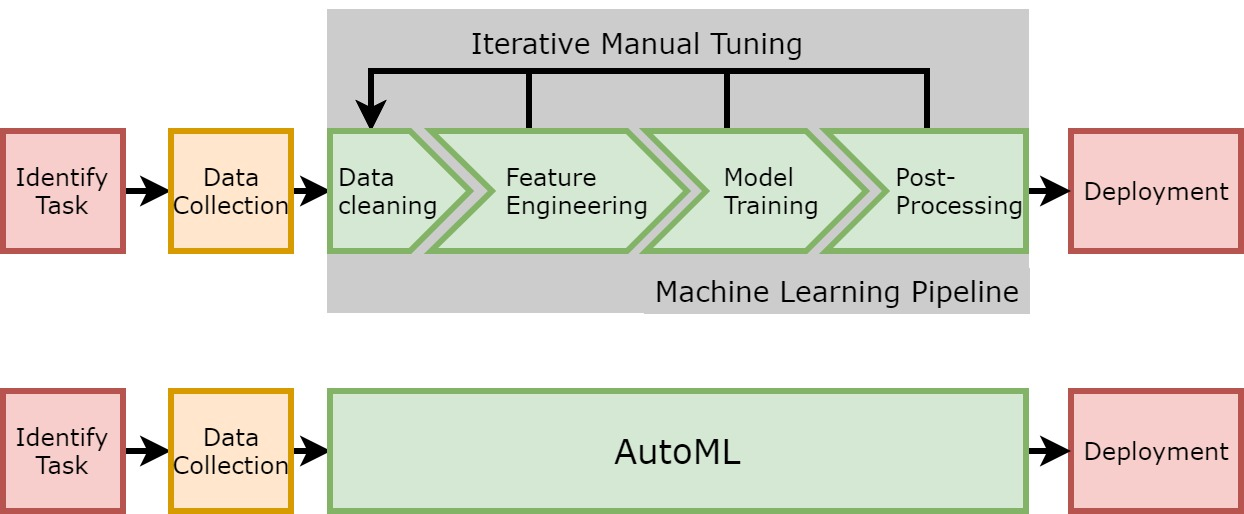
\includegraphics[width = \linewidth]{images/AutoMLPipeline.jpg}  
				\end{center}
			\end{column}
		\end{columns}
		
	\end{frame}
	
%	\begin{frame}{Preprocessing capabilities differ heavily}
%		\begin{columns}
%			\begin{column}{0.6\textwidth}
%				\vspace*{-1cm}
%				\begin{center}
%					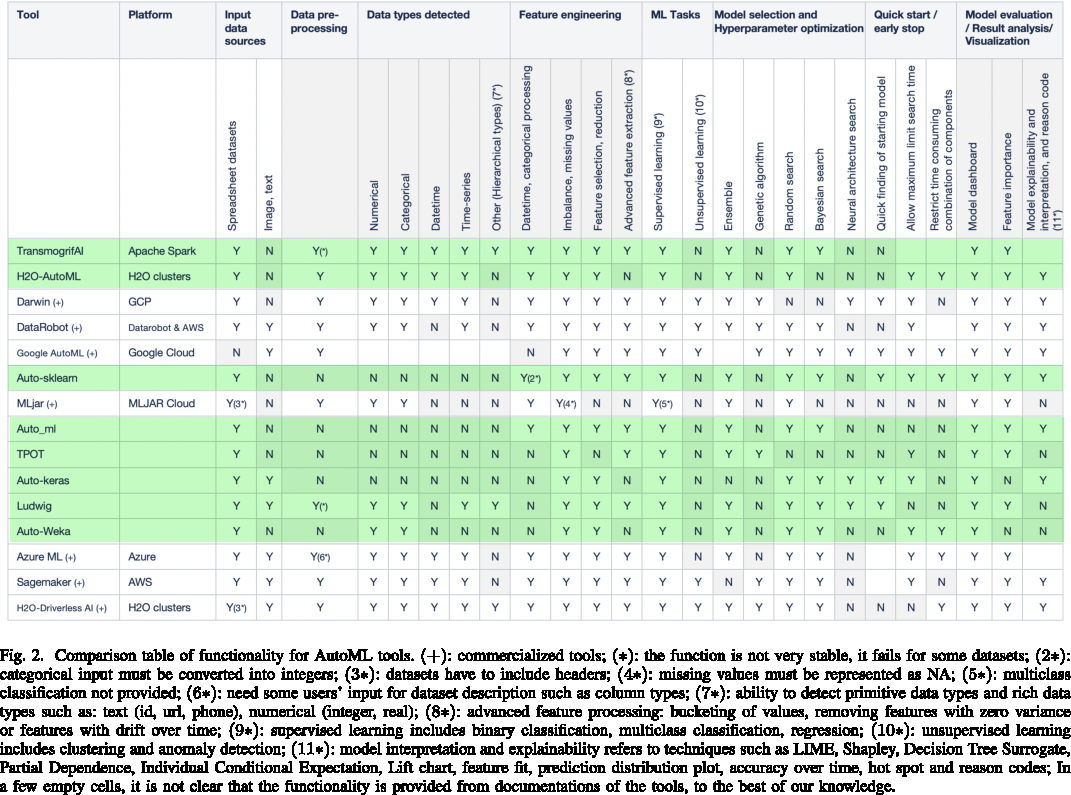
\includegraphics[width = \linewidth]{images/Truong2019Towards_fig2.pdf}
%				\end{center}
%				\vspace{-1em}
%				{\tiny Source~\lit{\href{https://doi.org/10.1109/ICTAI.2019.00209}{Truong et al. 2019}}.}
%			
%			\end{column}%
%			\begin{column}{0.4\textwidth}
%				\small
%				
%				\vspace{1em}
%				
%				Highlighted: Non-commercial AutoML frameworks
%				
%				\begin{itemize}
%					\item Auto-detection of feature types: some
%					\item Preprocess categoricals: some
%					\item Imputation: all
%					\item Class imbalance handling: all
%				\end{itemize}
%			\end{column}
%		\end{columns}
%	\end{frame}
	
	\begin{frame}{Simple Preprocessing and Cleaning}
		\begin{itemize}
			\item Data cleaning is hard to fully automate since errors in the data can be semantic.
			\item A few simple things should always be done:
			\pause
			\begin{itemize}
				\item Remove ID columns, columns with only unique values
				\item Remove duplicated columns
				\item Remove constant columns
			\end{itemize}
			\pause
			\item Already harder, but still possible:
			\begin{itemize}
				\item Detect outliers
				\item Detect correct column types (numeric, discrete, datetime, ...)
				\item Detect missing value encoding
			\end{itemize}
			\pause
			\item Even harder:
			\begin{itemize}
				\item Detect spelling and formatting errors
				\item Detect inconsistencies (e.g. zip code does not match city name)
				\item Detect time series or spatial data 
			\end{itemize}  
		\end{itemize}

		
		It is unclear how much of this is required input by the user (last point is more or less task specification) and what should be automated by the system. 
		
	\end{frame}

	\begin{frame}{Preprocessing: Categorical Features}
	
	\textit{Categorical} features have a fixed number of distict (unordered) possible values called levels.  

	\vspace{0.5cm}

		\begin{itemize}
			\item For most learners categorical features need to be encoded in numeric features.
			\item Distinguish between binary, low cardinality and high cardinality categorical features. Low or high cardinality refers to the number of levels.
			\begin{itemize}
				\item Binary: Encode as $1-0$.
				\item Low-cardinality: One-hot encoding.
				\item High-cardinality: Regularized target/impact encoding, clustering, hashing.
			\end{itemize}
			\item Tree-based algorithms (in some software implementations) can natively handle even high-cardinality categorical features.
			\item Optimal encoding can vary between each feature, algorithm and hyperparameter configuration. Introduce and tune threshold hyperparameter that decides when to use high-cardinality encoding, e.g. $n_{lvls} \ge \tau_{\text{high card.}}$.
			\item The encoder should also be able to handle new feature levels occuring at test time without crashing. 
		\end{itemize}
	\end{frame}


%	\begin{frame}{Categorical Features: Dummy Encoding}
%		% Goals:
%		\begin{itemize}
%			\item Most simple encoding
%			\item Works well with low cardinality categoricals
%		\end{itemize}
%		% ML algorithm does not support categorical features + few unique values $\rightarrow$ use dummy encoding.
%		% Most simple technique to encode categ
%		\begin{center}
%			\resizebox{0.3\linewidth}{!}{
%				\begin{tabular}{r|l|l}
%					\hline
%					SalePrice & Central.Air & Bldg.Type\\
%					\hline
%					189900 & Y & 1Fam\\
%					\hline
%					195500 & Y & 1Fam\\
%					\hline
%					213500 & Y & TwnhsE\\
%					\hline
%					191500 & Y & TwnhsE\\
%					\hline
%					236500 & Y & TwnhsE\\
%					\hline
%				\end{tabular}
%			} \\
%			\begin{tikzpicture}
%				%\useasboundingbox (-2,0);
%				\node[single arrow,draw=black,fill=black!10,minimum height=1cm,shape border rotate=270] at (0,-1) {};
%			\end{tikzpicture} \\
%			\resizebox{0.9\linewidth}{!}{
%				\begin{tabular}{r|r|r|r|r|r}
%					\hline
%					SalePrice & Y & Bldg.Type.2fmCon & Bldg.Type.Duplex & Bldg.Type.Twnhs & Bldg.Type.TwnhsE\\
%					\hline
%					189900 & 1 & 0 & 0 & 0 & 0\\
%					\hline
%					195500 & 1 & 0 & 0 & 0 & 0\\
%					\hline
%					213500 & 1 & 0 & 0 & 0 & 1\\
%					\hline
%					191500 & 1 & 0 & 0 & 0 & 1\\
%					\hline
%					236500 & 1 & 0 & 0 & 0 & 1\\
%					\hline
%				\end{tabular}
%			}
%		\end{center}
%	\end{frame}
%	
%	\begin{frame}{Categorical Features: Target / Impact Encoding}
%		\begin{itemize}
%			\item Well known from CART
%			\item Handles high cardinality categoricals, too
%		\end{itemize}
%		
%		% Avoid high cardinality categorical features because they are problematic for all ML algorithms $\rightarrow$ use target encoding (also impact encoding).
%		\begin{columns}
%			\begin{column}{0.3\textwidth}
%				\vspace{-2em}
%				\begin{center}
%					%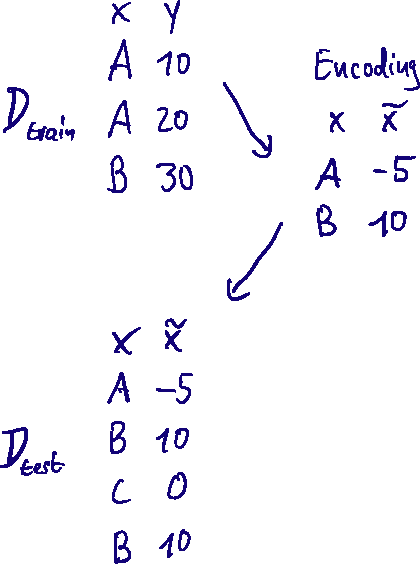
\includegraphics[width = \textwidth]{images/scetch_impact_encoding.pdf}
%					\resizebox{0.8\columnwidth}{!}{
%						\begin{tikzpicture}
%							\path
%							(0,1) coordinate (A) node[above, inner sep=0] {
%								\begin{tabular}{ c c }
%									\multicolumn{2}{ c }{$\dataset_{\text{train}}$} \\
%									%\hline
%									$x$ & $y$  \\
%									\hline
%									A & 10 \\
%									A & 20 \\
%									B & 30 \\
%								\end{tabular}
%							}
%							(0,-1) coordinate (B) node[below, inner sep=0] {
%								\begin{tabular}{ c c }
%									\multicolumn{2}{ c }{$\dataset_{\text{test}}$} \\
%									%\hline
%									x & $\tilde{x}$  \\
%									\hline
%									A & -5 \\
%									B & 10 \\
%									C & 0 \\
%								\end{tabular}
%							}
%							(1,0) coordinate (C) node[right, inner sep=0] {
%								\begin{tabular}{ c c }
%									\multicolumn{2}{ c }{Encoding} \\
%									%\hline
%									$x$ & $\tilde{x}$  \\
%									\hline
%									A & -5 \\
%									B & 10 \\
%								\end{tabular}
%							};
%							%\draw[->] (A)--(B) (0,0) -- node[above]{}(C);
%							\draw[myarrow, shorten <=0.1cm, shorten >=0.1cm] (A.south)--(C.north);
%							\draw[myarrow, shorten <=0.1cm, shorten >=0.1cm] (C.south)--(B.north);
%						\end{tikzpicture}
%					}
%				\end{center}
%			\end{column}
%			\begin{column}{0.7\textwidth}
%				
%				
%				\textbf{Goal}: Encodes each categorical $\bm{x}$ as a single numeric $\tilde{\bm{x}}$
%				
%				\vspace*{-0.5cm}  
%				{\footnotesize
%					\begin{align*}
%						\text{Regression:} \operatorname{Impact}(x) &= \E(\bm{y} | x) - \E(\bm{y}) \\
%						\text{Classification:} \operatorname{Impact}(x) &= \operatorname{logit}(P( y = \text{target} | x)) - \operatorname{logit}(P( y = \text{target}))
%					\end{align*}
%				}
%				\vspace*{-0.5cm}  
%				\begin{itemize}
%					
%					\item Needs regularization (through CV) to prevent target leakage \lit{\href{https://arxiv.org/pdf/1611.09477.pdf}{Zumel et al. 2019}}
%					
%					\item Advantage: Handles unknown categorical levels on test data
%				\end{itemize}
%				\pause
%				Alternatives: 
%				\begin{itemize}
%					\item factorization machines 
%					\item clustering feature levels 
%					\item feature hashing
%				\end{itemize}
%			\end{column}%
%
%		\end{columns}
%	\end{frame}
	
\begin{frame}{Preprocessing: Missing Values}

	\textit{Imputation} is the process of replacing missing values with artificial substituted values.

	\vspace{0.5cm}

	\begin{itemize}
		\item Simple imputation techniques replace missings with the mean, median, mode or a sample from empirical distribution of the feature.
		\item To keep track of the imputation, binary indicator features are added.
		\item For categorical features, missing values can easily be replaced by a new seperate level.
		\item Tree-based algorithms (in some software implementations) can natively handle missing values.
		\item Model-based imputation trains a machine learning model $f(x_{-i}) = x_i$ to predict missing values of $x_i$ using the remaining features $x_{-i} = x_1, ..., x_{i-1}, x_{i+1}, ..., x_p$.
		\begin{itemize}
			\item The imputation model should be able to handle missings natively.
			\item The choice of learner and its hyperparameters add additional complexity to the imputation.
			\item Random Forests are a reasonable choice.
		\end{itemize}
	\end{itemize}

\end{frame}

\begin{frame}{Feature Engineering}
	\begin{columns}
		\begin{column}{0.6\textwidth}
			\begin{itemize}
				\item $1:1$ Transformations
				\begin{itemize}
					\item $\log$, $\sqrt{\cdot}$, ....
					\item Standardization, Box-Cox, 0-1-scaling, ...
					\item Binning of numeric features 
				\end{itemize}
				\item $1:many$ Transformations
				\begin{itemize}
					\item Polynomial expansion: $x_j \longrightarrow x_j, x_j^2, x_j^3, ...$
					\item Basis expansions with B/P-splines
					\item Transform to ``circular'' features (month, day)\\ e.g.\ $\tilde x_1 = sin(2\pi \cdot x_1 /24)$
					\item Extract Weekday/Day/... from datetime features
				\end{itemize}
				\item $many:many$ Transformations 
				\begin{itemize}
					\item (kernel) Principal component analysis
					\item Truncated singular value decomposition
					\item Idependent component analysis
					\item Autoencoder
				\end{itemize}
			\end{itemize}
	\end{column}%
	\begin{column}{0.4\textwidth}
		\begin{center}
			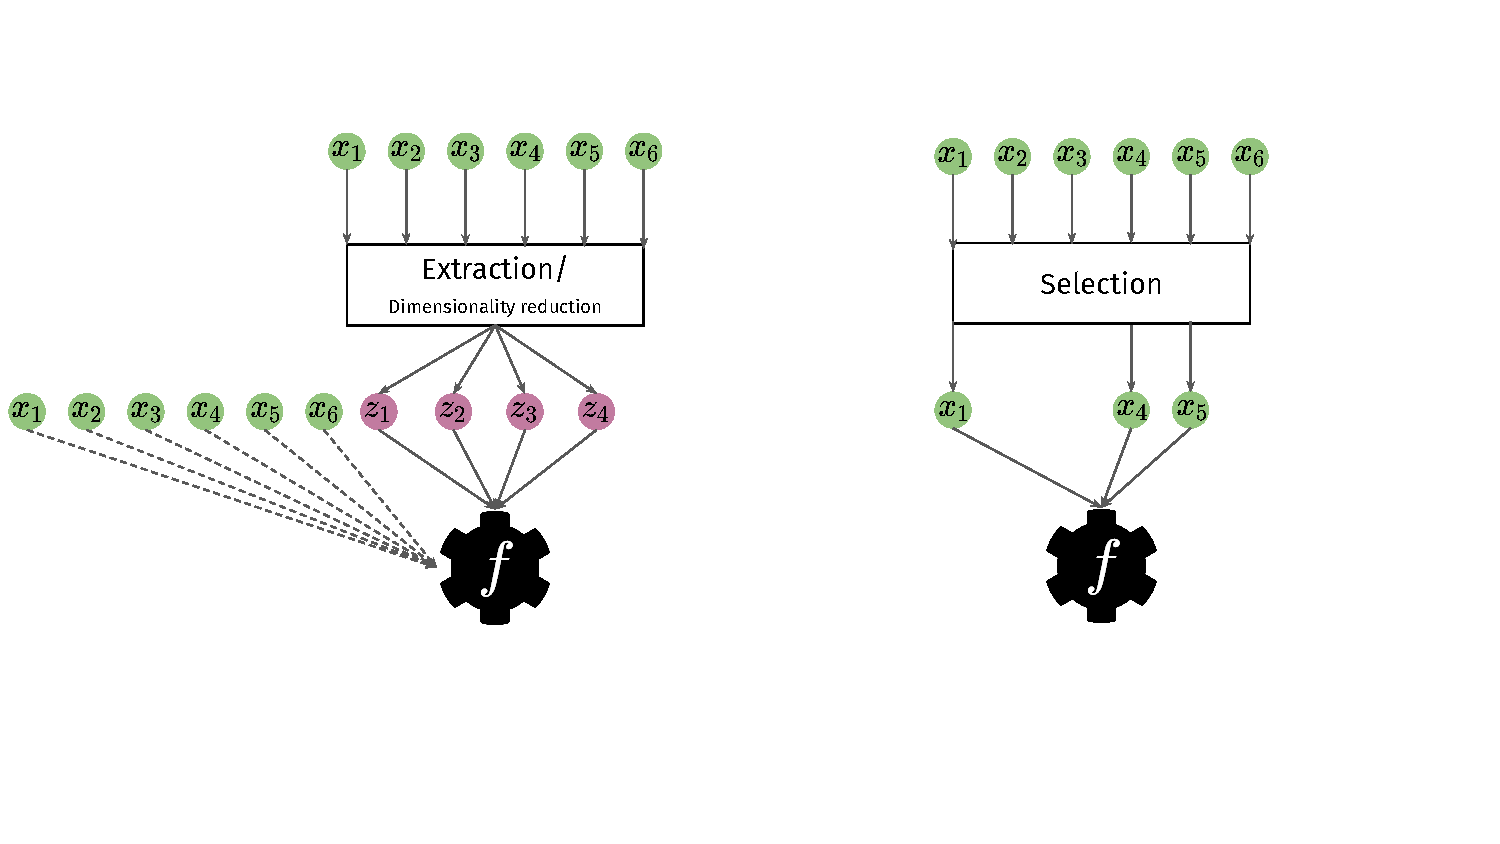
\includegraphics[width= \textwidth, trim=0 100 390 60, clip]{images/feat_extr_vs_selection.pdf}
			\end{center}
	\end{column}
	\end{columns}
\end{frame}

	\begin{frame}{Feature Selection}
		\begin{columns}
			\begin{column}{0.6\textwidth}
				\begin{itemize}
					
					\item Feature filter rank features and select most important fraction.
					\item Stepwise / wrapper methods greedily select one feature after another. 
					\item Some learner have embedded feature selection CART, lasso, \ldots 
					\item $p$-dimensional bitvector as hyperparameters.
					\item Combined feature selection and HPO: \lit{\href{hhttps://dl.acm.org/doi/abs/10.1145/3377930.3389815}{Binder et al. 2020}}
					
				\end{itemize}
			\end{column}%
			\begin{column}{0.4\textwidth}
				\begin{center}
					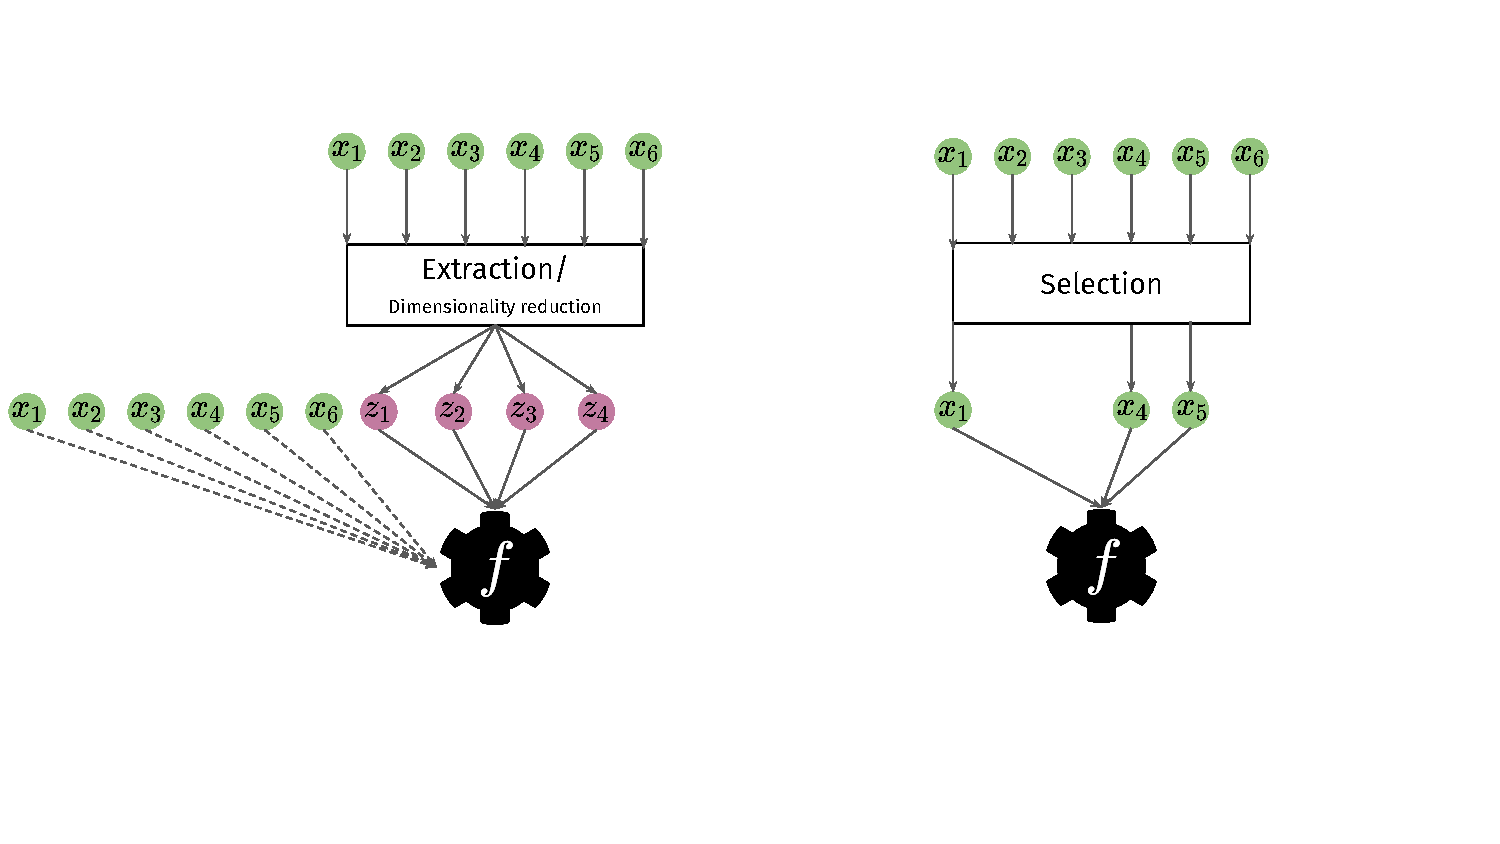
\includegraphics[width=0.5\textwidth, trim=450 100 110 60, clip]{images/feat_extr_vs_selection.pdf}%
					\end{center}
			\end{column}
		\end{columns}
		
	\end{frame}
	

	
	
	\begin{frame}{Imbalanced Classes}
	
		\textit{Imbalanced} classifcation occurs if one (usually more important) class appears much less frequent than other classes.

		\begin{columns}
			\begin{column}{0.6\textwidth}
				\begin{itemize}
					\item Tune class weights as hyperparameters.
					\item Undersmpling of majority class.
					\item Oversampling of minority class or generating synthetic samples (e.g. SMOTE).
					\item Pitfall: Be careful with resampling and ensure stratification.
					\item Pitfall: Rebalancing can create poorly calibrated models.
					\item If imbalance is severe change framing, e.g. anomaly detection.
				\end{itemize}
			\end{column}%
			\begin{column}{0.4\textwidth}
				\begin{center}
					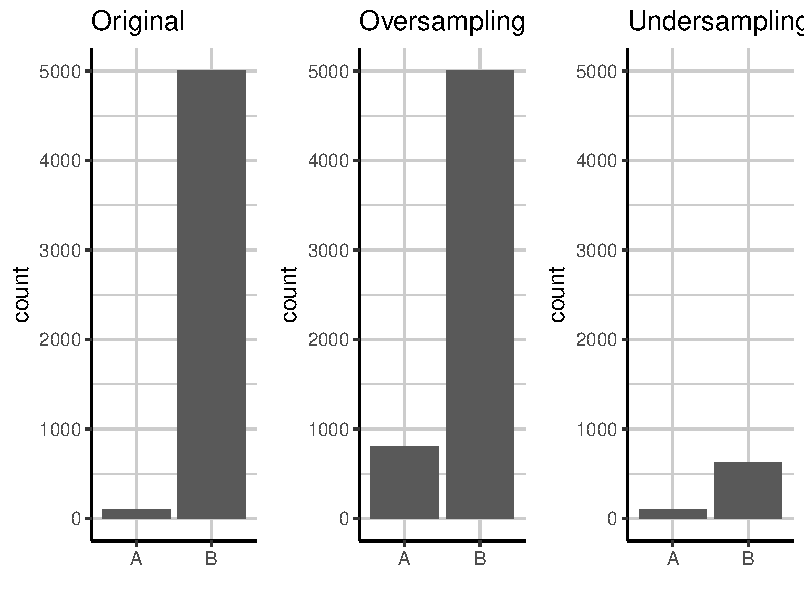
\includegraphics[width=0.8\textwidth]{images/imbalanced_resampling.pdf}
				\end{center}
			\scriptsize{Rebalancing for a binary classification problem with classes \texttt{A} and \texttt{B}.}
			\end{column}
		\end{columns}
	\end{frame}
	
	
	
\end{document}
